\documentclass[aspectratio=1610,onlymath]{beamer}
% \documentclass[aspectratio=1610,onlymath,handout]{beamer}

\input{macros-lecture}
% Common notation

\usepackage{amsmath,amssymb,amsfonts}
\usepackage{xspace}

\newcommand{\lectureurl}{https://iccl.inf.tu-dresden.de/web/FS2023}

\DeclareMathAlphabet{\mathsc}{OT1}{cmr}{m}{sc} % Let's have \mathsc since the slide style has no working \textsc

% Dual of "phantom": make a text that is visible but intangible
\newcommand{\ghost}[1]{\raisebox{0pt}[0pt][0pt]{\makebox[0pt][l]{#1}}}

\newcommand{\tuple}[1]{\langle{#1}\rangle}
\newcommand{\defeq}{\mathrel{:=}}

%%% Annotation %%%

\usepackage{color}
\newcommand{\todo}[1]{{\tiny\color{red}\textbf{TODO: #1}}}



%%% Old macros below; move when needed

\newcommand{\blank}{\text{\textvisiblespace}} % empty tape cell for TM

% table syntax
\newcommand{\dom}{\textbf{dom}}
\newcommand{\adom}{\textbf{adom}}
\newcommand{\dbconst}[1]{\texttt{"#1"}}
\newcommand{\pred}[1]{\textsf{#1}}
\newcommand{\foquery}[2]{#2[#1]}
\newcommand{\ground}[1]{\textsf{ground}(#1)}
% \newcommand{\foquery}[2]{\{#1\mid #2\}} %% Notation as used in Alice Book
% \newcommand{\foquery}[2]{\tuple{#1\mid #2}}

\newcommand{\quantor}{\mathord{\reflectbox{$\text{\sf{Q}}$}}} % the generic quantor

% logic syntax
\newcommand{\Inter}{\mathcal{I}} %used to denote an interpretation
\newcommand{\Jnter}{\mathcal{J}} %used to denote another interpretation
\newcommand{\Knter}{\mathcal{K}} %used to denote yet another interpretation
\newcommand{\Zuweisung}{\mathcal{Z}} %used to denote a variable assignment

% query languages
\newcommand{\qlang}[1]{{\sf #1}} % Font for query languages
\newcommand{\qmaps}[1]{\textbf{QM}({\sf #1})} % Set of query mappings for a query language

%%% Complexities %%%

\hyphenation{Exp-Time} % prevent "Ex-PTime" (see, e.g. Tobies'01, Glimm'07 ;-)
\hyphenation{NExp-Time} % better that than something else

% \newcommand{\complclass}[1]{{\sc #1}\xspace} % font for complexity classes
\newcommand{\complclass}[1]{\ensuremath{\mathsc{#1}}\xspace} % font for complexity classes

\newcommand{\ACzero}{\complclass{AC$_0$}}
\newcommand{\LogSpace}{\complclass{L}}
\newcommand{\NLogSpace}{\complclass{NL}}
\newcommand{\PTime}{\complclass{P}}
\newcommand{\NP}{\complclass{NP}}
\newcommand{\coNP}{\complclass{coNP}}
\newcommand{\PH}{\complclass{PH}}
\newcommand{\PSpace}{\complclass{PSpace}}
\newcommand{\NPSpace}{\complclass{NPSpace}}
\newcommand{\ExpTime}{\complclass{ExpTime}}
\newcommand{\NExpTime}{\complclass{NExpTime}}
\newcommand{\ExpSpace}{\complclass{ExpSpace}}
\newcommand{\TwoExpTime}{\complclass{2ExpTime}}
\newcommand{\NTwoExpTime}{\complclass{N2ExpTime}}
\newcommand{\ThreeExpTime}{\complclass{3ExpTime}}
\newcommand{\kExpTime}[1]{\complclass{#1ExpTime}}
\newcommand{\kExpSpace}[1]{\complclass{#1ExpSpace}}


\usepackage{verbatim}

\defineTitle{11}{Von regulären zu kontextfreien Sprachen}{30. November 2020}

\begin{document}

\maketitle

% \sectionSlide{Viereinhalb Wochen\\reguläre Sprachen}

\frame{\begin{center}
\LARGE
Viereinhalb Wochen\\reguläre Sprachen
\bigskip

\normalsize
auf sieben Folien
\end{center}}

\begin{frame}\frametitle{Die Chomsky-Hierarchie}

\defbox{
Die \redalert{Chomsky-Hierarchie} unterteilt Grammatiken in vier Stufen:
\begin{itemize}
\item \emph{Typ 0}: beliebige Grammatiken
\item \emph{Typ 1}: \redalert{kontextsensitive Grammatiken}:\\
	\begin{enumerate}[(a)]
	\item Alle Regeln $w\to v$ erfüllen die Bedingung $|w|\leq|v|$.
	\item Es gibt eine Regel $\Snterm{S}\to\epsilon$ und alle anderen Regeln $w\to v$ enthalten kein $\Snterm{S}$ in $v$ und erfüllen $|w|\leq|v|$.
	\end{enumerate}
\item \emph{Typ 2}: \redalert{kontextfreie Grammatiken}:\\
	Alle Regeln haben die Form $\Snterm{A}\to v$ für eine Variable $\Snterm{A}$.
\item \emph{Typ 3}: \redalert{reguläre Grammatiken}:\\
	Alle Regeln haben eine der Formen
	\[ \Snterm{A}\to \Sterm{c}\Snterm{B}\qquad \Snterm{A}\to \Sterm{c} \qquad \Snterm{A}\to \epsilon\]
	wobei $\Snterm{A}$ und $\Snterm{B}$ Variablen sind und $\Sterm{c}$ ein Terminalsymbol ist.
\end{itemize}

}

\end{frame}

\begin{frame}\frametitle{Chomskys Hierarchie ist eine Hierarchie}

\begin{tikzpicture}[decoration=penciline, decorate]
\node (nl) [decorate,draw=nightblue, text depth = 4cm, text width = \linewidth, fill=nightblue!10,thick,align=left, inner ysep=2mm, inner xsep=2mm] at (0,0) {Formale Sprachen};
\node (n0) [decorate,draw=darkgreen, text depth = 3cm, text width = 8cm, fill=darkgreen!10,thick,align=left, inner ysep=2mm, inner xsep=2mm] at ([yshift=-0.5em]nl.center) {Typ-0-Sprachen};
\node (n1) [decorate,draw=strongyellow, text depth = 2cm, text width = 6.7cm,  fill=strongyellow!10,thick,align=left, inner ysep=2mm, inner xsep=2mm] at ([yshift=-0.5em]n0.center) {Kontextsensitive Sprachen (Typ 1)};
\node (n2) [decorate,draw=orange, text depth = 1cm, text width = 5.4cm,  fill=orange!10,thick,align=left, inner ysep=2mm, inner xsep=2mm] at ([yshift=-0.5em]n1.center) {Kontextfreie Sprachen (Typ 2)};
\node (n3) [decorate,draw=red, fill=red!10,thick,align=left, inner ysep=2mm, inner xsep=2mm] at ([yshift=-0.5em]n2.center) {Reguläre Sprachen (Typ 3)};
\end{tikzpicture}
% \bigskip

(Dafür mussten wir Typ-1 erweitern und $\epsilon$-Regeln bei Typ-2 eliminieren.)

\end{frame}

\begin{frame}\frametitle{Automaten}

Wir kennen mehrere \alert{Varianten endlicher Automaten}:
\begin{itemize}
\item \redalert{Deterministischer endlicher Automat (DFA)}
	\begin{itemize}
	\item mit totaler Übergangsfunktion
	\end{itemize}
\item \redalert{Nichtdeterministischer endlicher Automat (NFA)}
	\begin{itemize}
	\item mit $\epsilon$-Übergängen
	\item mit Wortübergängen
	\item mit Übergängen für reguläre Ausdrücke (nur für Umwandlung reg.\ Ausdruck $\to$ $\epsilon$-NFA)
	\end{itemize}
\end{itemize}\medskip

Die \alert{Sprache eines Automaten} haben wir auf zwei Arten definiert
\begin{itemize}
\item Mithilfe einer verallgemeinerten Übergangsfunktion, die ganze Wörter einliest
\item Durch akzeptierende Läufe, die einem Wort zugeordnet werden können
\end{itemize}

\end{frame}

\begin{frame}[fragile]\frametitle{Darstellungen von Typ-3-Sprachen}

\mbox{}\hspace{-0cm}%
\begin{tikzpicture}[
	decoration=penciline, decorate,
	node distance = 7mm and 9mm,
	mybox/.style args = {#1/#2}{
		draw=#1,% line color
		fill=#2,% fill color
% 		rounded corners,
		thick,
		text width=18mm, minimum height=12mm, inner sep=1mm,
		align=flush center
	},
	myboxlabel/.style args = {}{
		draw=devilscss,% line color
		fill=strongyellow!40,% fill color
% 		rounded corners,
		thick,
		text width=17mm, minimum height=10mm, inner sep=1.5mm,
		align=flush center
	},
	myarrow/.style args = {#1}{
		line width=0.8mm,
		draw=#1,%line color
		%-{Triangle[length=2.8mm,width=4mm,fill=#1]},
		->,
		shorten >=0.5mm, shorten <=0.1mm
	}
]
\pgfmathsetseed{7729}
% \draw[help lines] (0,0) grid (5,5);
\node (reg) [decorate,mybox=black/cyan!40] at (2,-0.6) {reguläre Grammatik};
\node (dfa) [decorate,mybox=black/cyan!40] at (0,-4) {DFA};
\node (nfa) [decorate,mybox=black/cyan!40] at (4,-4) {NFA};
\node (re) [decorate,mybox=black/cyan!40] at (6,-0.6) {regulärer Ausdruck};
\node (enfa) [decorate,mybox=black/cyan!40] at (8,-4) {$\epsilon$-NFA};
%
\path[myarrow=devilscss,bend left=20](dfa) edge (reg.180);
% \node (dfareglabel) [decorate,myboxlabel=,text width=19mm] at (-0.4,-0.7) {"`$q_1 \stackrel{\Sterm{a}}{\to} q_2$"' $\leadsto$ "`$q_1\to\Sterm{a}q_2$"'};
%
\path[myarrow=devilscss,-,bend left=20](reg.340) edge[->] (nfa.110);
\path[myarrow=devilscss,-,bend right=20](nfa.130) edge[->] (reg.320);
\node (regnfalabel) [decorate,myboxlabel=] at (1.6,-1.9) {\footnotesize"`$q_1\to\Sterm{a}q_2$"' $\Leftrightarrow$ "`$q_1 \stackrel{\Sterm{a}}{\to} q_2$"'};
%
\draw[myarrow=devilscss](dfa.10)--(nfa.170);
\node (dfanfalabel) [decorate,myboxlabel=,text width=16mm, minimum height=5mm,inner sep=1mm] at (1.95,-3.3) {\scalebox{0.8}{"`DFA${}\subseteq{}$NFA"'}};
%
\draw[myarrow=devilscss](nfa.190)--(dfa.350);
\node (nfadfalabel) [decorate,myboxlabel=,text width=13mm] at (2.1,-5.0) {\footnotesize Potenzm.\-konstr.};
%
\node (sd) [decorate,mybox=black/cyan!40,text width=14mm, minimum height=10mm] at (4,-6.5) {\footnotesize Syntax\-diagramm};
\draw[myarrow=devilscss,<->](sd)--(nfa);
\node (sdnfalabel) [decorate,myboxlabel=, minimum height=0mm,inner sep=1.0mm,text width=19mm] at (5.3,-5.4) {\footnotesize dualer Graph};
%%
\path[myarrow=devilscss,-,bend left=20](nfa.70) edge[->] (re.180);
%
\path[myarrow=devilscss,-,bend left=20](re.0) edge[->] (enfa);
%
\draw[myarrow=devilscss](enfa.190)--(nfa.350);
\draw[myarrow=devilscss](nfa.10)--(enfa.170);
\node (nfaenfalabel) [decorate,myboxlabel=,text width=16mm, minimum height=5mm,inner sep=1mm] at (5.95,-3.3) {\scalebox{0.75}{"`NFA${}\subseteq{}${}$\epsilon$-NFA"'}};
\node (enfanfalabel) [decorate,myboxlabel=,text width=13mm, minimum height=5mm] at (6.1,-4.6) {\footnotesize $\epsilon$-Elim.};
%
\node (nfarelabel) [decorate,myboxlabel=,align=flush left,text width=17mm,inner sep=1mm] at (8.6,-0.7) {\footnotesize 1) komposit.\\2) explizit};

%
\node (reenfalabel) [decorate,myboxlabel=,align=flush left,text width=18mm,inner sep=1mm] at (5.6,-2.0) {\footnotesize 1) Ersetzung\\2) Dyn. Prog.};
\end{tikzpicture}

\end{frame}

\newcommand{\simquot}[1]{#1/_{\!\!{\sim}}}

\begin{frame}\frametitle{Umformungsalgorithmen (1)}

\begin{tabular}{@{}rll@{}}
\emph{Eingabe} & \emph{Ausgabe} & \emph{Vorlesung} \\
kontextfreie Grammatik & $\epsilon$-freie kontextfreie Grammatik & 2\\
DFA $\Smach{M}$ & totaler DFA $\Smach{M}_{\text{total}}$ & 3\\
DFA $\Smach{M}$ & reguläre Grammatik $G_{\Smach{M}}$ & 3\\
Syntaxdiagramm & NFA & 4\\
NFA $\Smach{M}$ & Potenzmengen-DFA $\Smach{M}_{\text{DFA}}$ & 4\\
reguläre Grammatik $G$ & NFA $\Smach{M}_G$ & 5\\
NFA mit Wortübergängen & $\epsilon$-NFA & 5\\
$\epsilon$-NFA $\Smach{M}$ & NFA $\textsf{elim}_\epsilon(\Smach{M})$ & 5
\end{tabular}

\end{frame}

\begin{frame}\frametitle{Umformungsalgorithmen (2)}

\begin{tabular}{@{}rll@{}}
\emph{Eingabe} & \emph{Ausgabe} & \emph{Vorlesung} \\
NFAs $\Smach{M}_1$, $\Smach{M}_2$ & Vereinigungs-NFA $\Smach{M}_1\oplus\Smach{M}_2$ & 5\\
NFAs/DFAs $\Smach{M}_1$, $\Smach{M}_2$ & Produkt-NFA/DFA $\Smach{M}_1\otimes\Smach{M}_2$ & 5\\
totaler DFA $\Smach{M}$ & Komplement-DFA $\overline{\Smach{M}}$ & 5\\
NFAs $\Smach{M}_1$, $\Smach{M}_2$ & $\epsilon$-NFA $\Smach{M}_1\odot\Smach{M}_2$ für Konkatenation & 5\\
NFA $\Smach{M}$ & $\epsilon$-NFA $\Smach{M}^*$ für Kleene-Abschluss & 5\\
regulärer Ausdruck & $\epsilon$-NFA (Komposition) & 6 \\
regulärer Ausdruck & $\epsilon$-NFA (explizit) & 6 \\
NFA & regulärer Ausdruck (Gleichungssystem) & 7 \\
NFA & regulärer Ausdruck (dyn. Programmierung) & 7 \\
totaler DFA $\Smach{M}$ & Quotienten-DFA $\simquot{\Smach{M}}$ & 8 \\
totaler DFA $\Smach{M}$ & reduzierter DFA $\Smach{M}_r$ & 8
\end{tabular}

\end{frame}

\begin{frame}\frametitle{Reguläre Sprachen}

\theobox{%
Die Menge der regulären Sprachen ist \ldots

\begin{itemize}
\item die Menge genau all jener Sprachen \ldots 
	\begin{itemize}
	\item die von einer Typ-3-Grammatik beschrieben werden
	\item die von einem DFA erkannt werden
	\item die von einem NFA erkannt werden
	\item die durch einen regulären Ausdruck beschrieben werden
	\item die endlich viele Myhill-Nerode-Kongruenzklassen haben
	\end{itemize}
\item die kleinste Menge von Sprachen \ldots
	\begin{itemize}
	\item welche alle endlichen Sprachen enthält und unter $\cap$, $\cup$, $\overline{\phantom{L}}$, $\circ$ und ${}^*$ abgeschlossen ist
	\item welche die Sprachen $\emptyset$, $\{\epsilon\}$ und $\{\Sterm{a}\}$ ($\Sterm{a}\in\Sigma$) enthält und unter $\cup$, $\circ$ und ${}^*$ abgeschlossen ist
	\end{itemize}
\end{itemize}}

Alle endlichen Sprachen sind regulär (aber nicht umgekehrt)\\
Alle regulären Sprachen erlauben Pumping (aber nicht umgekehrt)

\end{frame}


\begin{frame}\frametitle{Probleme für endliche Automaten}

\begin{tabular}{@{}rll@{}}
\emph{Problem} & \emph{Fragestellung} & \emph{Komplexität} \\[1ex]
Leerheit & $\Slang{L}(\Smach{M})\stackrel{?}{=}\emptyset$  & polynomiell\\[1ex]
Inklusion & $\Slang{L}(\Smach{M}_1)\stackrel{?}{\subseteq}\Slang{L}(\Smach{M}_2)$  & polynomiell falls $\Smach{M}_2$ DFA\\[-0.5ex]
	& & exponentiell falls $\Smach{M}_2$ NFA\\[1ex]
Äquivalenz & $\Slang{L}(\Smach{M}_1)\stackrel{?}{=}\Slang{L}(\Smach{M}_2)$  & polynomiell falls $\Smach{M}_1$ und $\Smach{M}_2$ DFA\\[-0.5ex]
	& & exponentiell falls $\Smach{M}_1$ oder $\Smach{M}_2$ NFA\\[1ex]
Wortproblem & $w\stackrel{?}{\in}\Slang{L}(\Smach{M})$  & polynomiell\\[1ex]
Universalität & $\Slang{L}(\Smach{M})\stackrel{?}{=}\Sigma^*$  & polynomiell falls $\Smach{M}$ DFA\\[-0.5ex]
	& & exponentiell falls $\Smach{M}$ NFA\\[1ex]
Endlichkeit & $\Slang{L}(\Smach{M})$ endlich? & polynomiell 
\end{tabular}

\end{frame}

\sectionSlide{Kontextfreie Sprachen}

\begin{frame}\frametitle{Kontextfreie Sprachen}

Wir hatten kontextfreie Sprachen wie folgt definiert:

\medskip
\defbox{Eine \redalert{kontextfreie Grammatik} (oder \redalert{Typ-2-Grammatik} oder \redalert{CFG}) enthält nur Regeln der Form
$\Snterm{A}\to v$, wobei $\Snterm{A}$ eine Variable ist.\medskip

Eine  Sprache ist \redalert{kontextfrei} (oder \redalert{Typ 2}), wenn sie durch eine kontextfreie Grammatik dargestellt werden kann.
}\medskip\pause

Das genügt, um nichtreguläre Sprachen darzustellen:

\examplebox{\emph{Beispiel:} Die Sprache $\{\Sterm{a}^n\Sterm{b}^n\mid n\geq 0\}$ ist kontextfrei, da sie durch die folgende CFG dargestellt werden kann:
\begin{align*}
\Snterm{S} & \to \epsilon \mid \Sterm{a}\Snterm{S}\Sterm{b}
\end{align*}
{\footnotesize(Übung: Beweise, dass die Grammatik wirklich diese Sprache darstellt.)}
}

\end{frame}

\begin{frame}\frametitle{Beispiel}

CFGs eignen sich zur Darstellung vollständig geklammerter Ausdrücke.
\bigskip

\examplebox{\emph{Beispiel:} Vollständig geklammerte reguläre Ausdrücke über Alphabet $\Sigma=\{\sigma_1, \ldots, \sigma_n\}$ sind als CFG über dem Alphabet $\Sigma\cup\{\Sterm{\emptyset},\Sterm{\epsilon},\Sterm{(},\Sterm{)},\Sterm{\mid},\Sterm{{}^*}\}$ darstellbar:
\begin{align*}
 \Snterm{S} & \to \Sterm{\emptyset} \mid \Sterm{\epsilon} \mid \Snterm{A} \mid \Sterm{(}\Snterm{S}\Snterm{S}\Sterm{)} \mid \Sterm{(}\Snterm{S}\Sterm{\mid}\Snterm{S}\Sterm{)}\mid \Sterm{(}\Snterm{S}\Sterm{)}\Sterm{{}^*}\\
 \Snterm{A} & \to \sigma_1\mid \ldots \mid \sigma_n
\end{align*}
}\bigskip

Allgemein ist die Beschreibung korrekt geklammerter Ausdrücke für viele Sprachen sehr wichtig, nicht zuletzt für Programmiersprachen

\end{frame}

\begin{frame}[fragile]\frametitle{Ein praktisches Beispiel \ldots}

\pause
Kontextfreie Grammatik für XML 1.1 (in W3C EBNF):

% \scalebox{0.3}{%
% \tiny
\linespread{0.6}
\fontsize{2.3}{4}\selectfont
\begin{verbatim}
[1]   document          ::= prolog element Misc* - Char* RestrictedChar Char*
[2]   Char              ::= [#x1-#xD7FF] | [#xE000-#xFFFD] | [#x10000-#x10FFFF] /* any Unicode character, excluding the surrogate blocks, FFFE, and FFFF. */
[2a]  RestrictedChar    ::= [#x1-#x8] | [#xB-#xC] | [#xE-#x1F] | [#x7F-#x84] | [#x86-#x9F]
[3]   S                 ::= (#x20 | #x9 | #xD | #xA)+
[4]   NameStartChar     ::= ":" | [A-Z] | "_" | [a-z] | [#xC0-#xD6] | [#xD8-#xF6] | [#xF8-#x2FF] | [#x370-#x37D] | [#x37F-#x1FFF] | [#x200C-#x200D] | [#x2070-#x218F] | [#x2C00-#x2FEF] | [#x3001-#xD7FF] | [#xF900-#xFDCF] | [#xFDF0-#xFFFD] | [#x10000-#xEFFFF]
[4a]  NameChar          ::= NameStartChar | "-" | "." | [0-9] | #xB7 | [#x0300-#x036F] | [#x203F-#x2040]
[5]   Name              ::= NameStartChar (NameChar)*
[6]   Names             ::= Name (#x20 Name)*
[7]   Nmtoken           ::= (NameChar)+
[8]   Nmtokens          ::= Nmtoken (#x20 Nmtoken)*
[9]   EntityValue       ::= '"' ([^%&"] | PEReference | Reference)* '"' | "'" ([^%&'] | PEReference | Reference)* "'"
[10]  AttValue          ::= '"' ([^<&"] | Reference)* '"' | "'" ([^<&'] | Reference)* "'"
[11]  SystemLiteral     ::= ('"' [^"]* '"') | ("'" [^']* "'")
[12]  PubidLiteral      ::= '"' PubidChar* '"' | "'" (PubidChar - "'")* "'"
[13]  PubidChar         ::= #x20 | #xD | #xA | [a-zA-Z0-9] | [-'()+,./:=?;!*#@$_%]
[14]  CharData          ::= [^<&]* - ([^<&]* ']]>' [^<&]*)
[15]  Comment           ::= '<!--' ((Char - '-') | ('-' (Char - '-')))* '-->'
[16]  PI                ::= '<?' PITarget (S (Char* - (Char* '?>' Char*)))? '?>'
[17]  PITarget          ::= Name - (('X' | 'x') ('M' | 'm') ('L' | 'l'))
[18]  CDSect            ::= CDStart CData CDEnd
[19]  CDStart           ::= '<![CDATA['
[20]  CData             ::= (Char* - (Char* ']]>' Char*))
[21]  CDEnd             ::= ']]>'
[22]  prolog            ::= XMLDecl Misc* (doctypedecl Misc*)?
[23]  XMLDecl           ::= '<?xml' VersionInfo EncodingDecl? SDDecl? S?'?>'
[24]  VersionInfo       ::= S 'version' Eq ("'" VersionNum "'" | '"' VersionNum '"')
[25]  Eq                ::= S? '=' S?
[26]  VersionNum        ::= '1.1'
[27]  Misc              ::= Comment | PI | S
[28]  doctypedecl       ::= '<!DOCTYPE' S Name (S ExternalID)? S? ('[' intSubset ']' S?)? '>'
[28a] DeclSep           ::= PEReference | S
[28b] intSubset         ::= (markupdecl | DeclSep)*
[29]  markupdecl        ::= elementdecl | AttlistDecl | EntityDecl | NotationDecl | PI | Comment
[30]  extSubset         ::= TextDecl? extSubsetDecl
[31]  extSubsetDecl     ::= ( markupdecl | conditionalSect | DeclSep)*
[32]  SDDecl            ::= #x20+ 'standalone' Eq (("'" ('yes' | 'no') "'") | ('"' ('yes' | 'no') '"'))
(Productions 33 through 38 have been removed.)
[39]  element           ::= EmptyElemTag
[40]  STag              ::= '<' Name (S Attribute)* S? '>'
[41]  Attribute         ::= Name Eq AttValue
[42]  ETag              ::= '</' Name S? '>'
[43]  content           ::= CharData? ((element | Reference | CDSect | PI | Comment) CharData?)*
[44]  EmptyElemTag      ::= '<' Name (S Attribute)* S? '/>'
[45]  elementdecl       ::= '<!ELEMENT' S Name S contentspec S? '>'
[46]  contentspec       ::= 'EMPTY' | 'ANY' | Mixed | children
[47]  children          ::= (choice | seq) ('?' | '*' | '+')?
[48]  cp                ::= (Name | choice | seq) ('?' | '*' | '+')?
[49]  choice            ::= '(' S? cp ( S? '|' S? cp )+ S? ')'
[50]  seq               ::= '(' S? cp ( S? ',' S? cp )* S? ')'
[51]  Mixed             ::= '(' S? '#PCDATA' (S? '|' S? Name)* S? ')*' | '(' S? '#PCDATA' S? ')'
[52]  AttlistDecl       ::= '<!ATTLIST' S Name AttDef* S? '>'
[53]  AttDef            ::= S Name S AttType S DefaultDecl
[54]  AttType           ::= StringType | TokenizedType | EnumeratedType
[55]  StringType        ::= 'CDATA'
[56]  TokenizedType     ::= 'ID' | 'IDREF' | 'IDREFS' | 'ENTITY' | 'ENTITIES' | 'NMTOKEN' | 'NMTOKENS'
[57]  EnumeratedType    ::= NotationType | Enumeration
[58]  NotationType      ::= 'NOTATION' S '(' S? Name (S? '|' S? Name)* S? ')'
[59]  Enumeration       ::= '(' S? Nmtoken (S? '|' S? Nmtoken)* S? ')'
[60]  DefaultDecl       ::= '#REQUIRED' | '#IMPLIED' | (('#FIXED' S)? AttValue)
[61]  conditionalSect   ::= includeSect | ignoreSect
[62]  includeSect       ::= '<![' S? 'INCLUDE' S? '[' extSubsetDecl ']]>'
[63]  ignoreSect        ::= '<![' S? 'IGNORE' S? '[' ignoreSectContents* ']]>'
[64]  ignoreSectContents::= Ignore ('<![' ignoreSectContents ']]>' Ignore)*
[65]  Ignore            ::= Char* - (Char* ('<![' | ']]>') Char*)
[66]  CharRef           ::= '&#' [0-9]+ ';' | '&#x' [0-9a-fA-F]+ ';'
[67]  Reference         ::= EntityRef | CharRef
[68]  EntityRef         ::= '&' Name ';'
[69]  PEReference       ::= '%' Name ';'
[70]  EntityDecl        ::= GEDecl | PEDecl
[71]  GEDecl            ::= '<!ENTITY' S Name S EntityDef S? '>'
[72]  PEDecl            ::= '<!ENTITY' S '%' S Name S PEDef S? '>'
[73]  EntityDef         ::= EntityValue| (ExternalID NDataDecl?)
[74]  PEDef             ::= EntityValue | ExternalID
[75]  ExternalID        ::= 'SYSTEM' S SystemLiteral | 'PUBLIC' S PubidLiteral S SystemLiteral
[76]  NDataDecl         ::= S 'NDATA' S Name
[77]  TextDecl          ::= '<?xml' VersionInfo? EncodingDecl S? '?>'
[78]  extParsedEnt      ::= TextDecl? content - Char* RestrictedChar Char*
[80]  EncodingDecl      ::= S 'encoding' Eq ('"' EncName '"' | "'" EncName "'" )
[81]  EncName           ::= [A-Za-z] ([A-Za-z0-9._] | '-')*
[82]  NotationDecl      ::= '<!NOTATION' S Name S (ExternalID | PublicID) S? '>'
[83]  PublicID          ::= 'PUBLIC' S PubidLiteral
\end{verbatim}
% }

\end{frame}

\begin{frame}[t,fragile]\frametitle{Beispiel Compiler}

\begin{tikzpicture}[
	decoration=penciline, decorate,
	node distance = 7mm and 9mm,
	mybox/.style args = {#1/#2}{
		draw=#1,% line color
		fill=#2,% fill color
% 		rounded corners,
		thick,
		text width=47mm, minimum height=8mm, inner sep=1mm, 
		align=flush center
	},
	myarrow/.style args = {#1}{
		line width=0.8mm,
		draw=#1,%line color
		%-{Triangle[length=2.8mm,width=4mm,fill=#1]},
		->,
		shorten >=0.5mm, shorten <=0.1mm
	},
	myarrowb/.style args = {#1}{
		line width=0.3mm,
		draw=#1,%line color
		%-{Triangle[length=2.8mm,width=4mm,fill=#1]},
		->,
		shorten >=1mm, shorten <=0.1mm
	}
]
\pgfmathsetseed{7729}
% \draw[help lines] (0,0) grid (5,5);
\node (n1) [decorate,mybox=black/cyan!40] at (0,6) {Quellprogramm};
{
\node (n2) [decorate,mybox=black/white] at (0,4.5) {Lexer};
	\node (t2) [right=of n2,align=left] {\alert{lexikalische Analyse}\\erzeugt Folge von Tokens\\$\leadsto$ \redalert{reguläre Sprache}};
\node (n3) [decorate,mybox=black/white] at (0,3) {Parser};
	\node (t3) [right=of n3,align=left] {\alert{syntaktische Analyse}\\erzeugt Strukturbaum\\$\leadsto$ \redalert{kontextfreie Sprache}};
\node (n4) [decorate,mybox=black/white] at (0,1.5) {$\ldots$};
	\node (t4) [right=of n4,align=left] {Codeerzeugung,\\Optimierung,\ldots};
}
\node (n5) [decorate,mybox=black/cyan!40] at (0,0) {Programm in Zielsprache};
%
\draw[myarrow=black]    (n1) edge[decorate] (n2);
{
\draw[myarrow=black]    (n2) edge[decorate] (n3);
\draw[myarrow=black]    (n3) edge[decorate] (n4);
}
\draw[myarrow=black]    (n4) edge[decorate] (n5);
%
{
\draw[myarrowb=alert]    (t2) edge[decorate] (n2);
\draw[myarrowb=alert]    (t3) edge[decorate] (n3);
\draw[myarrowb=alert]    (t4) edge[decorate] (n4);
}
\end{tikzpicture}

\end{frame}


\begin{frame}\frametitle{Wiederholung: Ableitung}

\defbox{Sei $\tuple{V,\Sigma,P,S}$ eine Grammatik.
Die \redalert{1-Schritt-Ableitungsrelation} ist eine binäre Relation \redalert{$\Rightarrow$}
zwischen Wörtern aus $(V\cup\Sigma)^*$, so dass $u \Rightarrow v$ genau dann wenn:\\[1ex]
%
\narrowcentering{$u=w_1\, x\, w_2 \text{ und } v=w_1\, y\, w_2 \text{ und es gibt eine Regel }x\to y\in P$}\\[1ex]
%
wobei $w_1,w_2,x,y\in (V\cup\Sigma)^*$ beliebige Wörter sind.}

\medskip

\defbox{%
Die \redalert{Ableitungsrelation $\Rightarrow^*$} ist der reflexive, transitive Abschluss von
$\Rightarrow$, das heißt $u \Rightarrow^* v$ genau dann wenn:\\[1ex]
%
\narrowcentering{$u=w_1\Rightarrow w_2\Rightarrow \ldots\Rightarrow w_{n-1}\Rightarrow w_n=v$}\\[1ex]
% \narrowcentering{$u=w_1$ und $w_1\Rightarrow w_2$ und $\cdots{}$ und $w_{n-1}\Rightarrow w_n$ und $w_n=v$}\\[1ex]
%
wobei $n\geq 1$ und $w_1,\ldots,w_n\in (V\cup\Sigma)^*$ beliebige Wörter sind.
% \narrowcentering{es gibt Wörter $w_1,\ldots,w_n\in (V\cup\Sigma)^*$ für $n\geq 1$, so dass}\\\narrowcentering{$u=w_1$, $v=w_n$ und $w_1\Rightarrow w_2\Rightarrow \ldots\Rightarrow w_n$}\\[1ex]
%
Insbesondere gilt $u\Rightarrow^* u$ für alle $u\in (V\cup\Sigma)^*$ (Fall $n=1$).
}

{\footnotesize \textcolor{devilscss}{Anmerkung: Der Begriff "`Herleitungsrelation"' ist auch gebräuchlich. Wir verwenden "`Ableitung"' und "`Herleitung"' synonym.\\
Anmerkung 2: Manche Autoren schreiben $\vdash$ statt $\Rightarrow$.}}

\end{frame}


\begin{frame}\frametitle{Beispiel}

Die Grammatik
% 
\begin{align*}
\Snterm{S} &\to \Snterm{A}\mid \Snterm{M}\mid \Snterm{V}\\
\Snterm{A} &\to \Sterm{(}\Snterm{S}\Sterm{+}\Snterm{S}\Sterm{)}\\
\Snterm{M} &\to \Sterm{(}\Snterm{S}\Sterm{*}\Snterm{S}\Sterm{)}\\
\Snterm{V} &\to \Sterm{x}\mid\Sterm{y}\mid\Sterm{z}
\end{align*}
% 
erzeugt zum Beispiel das Wort $\Sterm{(x*(y+z))}$ über die Ableitung:
% 
\begin{align*}
\Snterm{S} &\Rightarrow \Snterm{M}
	\Rightarrow \Sterm{(}\Snterm{S}\Sterm{*}\Snterm{S}\Sterm{)}
	\Rightarrow \Sterm{(}\Snterm{V}\Sterm{*}\Snterm{S}\Sterm{)}
	\Rightarrow \Sterm{(}\Sterm{x}\Sterm{*}\Snterm{S}\Sterm{)}
	\Rightarrow \Sterm{(}\Sterm{x}\Sterm{*}\Snterm{A}\Sterm{)}
	\Rightarrow \Sterm{(}\Sterm{x}\Sterm{*}\Sterm{(}\Snterm{S}\Sterm{+}\Snterm{S}\Sterm{)}\Sterm{)}\\
	&\Rightarrow \Sterm{(}\Sterm{x}\Sterm{*}\Sterm{(}\Snterm{V}\Sterm{+}\Snterm{S}\Sterm{)}\Sterm{)}
	\Rightarrow \Sterm{(}\Sterm{x}\Sterm{*}\Sterm{(}\Sterm{y}\Sterm{+}\Snterm{S}\Sterm{)}\Sterm{)}
	\Rightarrow \Sterm{(}\Sterm{x}\Sterm{*}\Sterm{(}\Sterm{y}\Sterm{+}\Snterm{V}\Sterm{)}\Sterm{)}
	\Rightarrow \Sterm{(}\Sterm{x}\Sterm{*}\Sterm{(}\Sterm{y}\Sterm{+}\Sterm{z}\Sterm{)}\Sterm{)}
\end{align*}



\end{frame}

\begin{frame}\frametitle{Ableitungen als Bäume}

\begin{minipage}{4cm}
Grammatik:
\begin{align*}
\Snterm{S} &\to \Snterm{A}\mid \Snterm{M}\mid \Snterm{V} &
\Snterm{A} &\to \Sterm{(}\Snterm{S}\Sterm{+}\Snterm{S}\Sterm{)} \\
\Snterm{M} &\to \Sterm{(}\Snterm{S}\Sterm{*}\Snterm{S}\Sterm{)} &
\Snterm{V} &\to \Sterm{x}\mid\Sterm{y}\mid\Sterm{z}
\end{align*}

Ableitung:
\begin{align*}
\Snterm{S} &\visible<2->{\Rightarrow \Snterm{M}}
	\visible<3->{\Rightarrow \Sterm{(}\Snterm{S}\Sterm{*}\Snterm{S}\Sterm{)}}
	\visible<4->{\Rightarrow \Sterm{(}\Snterm{V}\Sterm{*}\Snterm{S}\Sterm{)}}\\
	&\visible<5->{\Rightarrow \Sterm{(}\Sterm{x}\Sterm{*}\Snterm{S}\Sterm{)}}
	\visible<6->{\Rightarrow \Sterm{(}\Sterm{x}\Sterm{*}\Snterm{A}\Sterm{)}}\\
	&\visible<7->{\Rightarrow \Sterm{(}\Sterm{x}\Sterm{*}\Sterm{(}\Snterm{S}\Sterm{+}\Snterm{S}\Sterm{)}\Sterm{)}}
	\visible<8->{\Rightarrow \Sterm{(}\Sterm{x}\Sterm{*}\Sterm{(}\Snterm{V}\Sterm{+}\Snterm{S}\Sterm{)}\Sterm{)}}\\
	&\visible<9->{\Rightarrow \Sterm{(}\Sterm{x}\Sterm{*}\Sterm{(}\Sterm{y}\Sterm{+}\Snterm{S}\Sterm{)}\Sterm{)}}
	\visible<10->{\Rightarrow \Sterm{(}\Sterm{x}\Sterm{*}\Sterm{(}\Sterm{y}\Sterm{+}\Snterm{V}\Sterm{)}\Sterm{)}}\\
	&\visible<11->{\Rightarrow \Sterm{(}\Sterm{x}\Sterm{*}\Sterm{(}\Sterm{y}\Sterm{+}\Sterm{z}\Sterm{)}\Sterm{)}}
\end{align*}
\end{minipage}\hfill
\begin{minipage}{4.5cm}
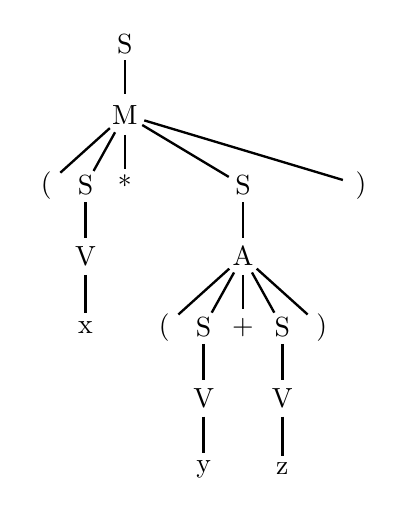
\begin{tikzpicture}[xscale=0.5,yscale=0.9,baseline={(current bounding box.center)}]
% \draw[help lines] (0,0) grid (7,2);
\node (s1) [circle,draw=none,inner sep=1pt] at (0,0) {\Snterm{S}};
\visible<2->{\node (s2) [circle,draw=none,inner sep=1pt] at (0,-1) {\Snterm{M}};}
\visible<3->{\node (s3) [circle,draw=none,inner sep=1pt] at (0,-2) {\Sterm{*}};
\node (s3a) [circle,draw=none,inner sep=1pt] at (3,-2) {\Snterm{S}};
\node (s3b) [circle,draw=none,inner sep=1pt] at (6,-2) {\Sterm{)}};
\node (s3x) [circle,draw=none,inner sep=1pt] at (-1,-2) {\Snterm{S}};
\node (s3y) [circle,draw=none,inner sep=1pt] at (-2,-2) {\Sterm{(}};}
\visible<6->{\node (s4) [circle,draw=none,inner sep=1pt] at (3,-3) {\Snterm{A}};}
\visible<4->{\node (s4z) [circle,draw=none,inner sep=1pt] at (-1,-3) {\Snterm{V}};}
\visible<7->{\node (s5) [circle,draw=none,inner sep=1pt] at (3,-4) {\Sterm{+}};
\node (s5a) [circle,draw=none,inner sep=1pt] at (4,-4) {\Snterm{S}};
\node (s5b) [circle,draw=none,inner sep=1pt] at (5,-4) {\Sterm{)}};
\node (s5x) [circle,draw=none,inner sep=1pt] at (2,-4) {\Snterm{S}};
\node (s5y) [circle,draw=none,inner sep=1pt] at (1,-4) {\Sterm{(}};}
\visible<5->{\node (s5z) [circle,draw=none,inner sep=1pt] at (-1,-4) {\Sterm{x}};}
\visible<10->{\node (s6a) [circle,draw=none,inner sep=1pt] at (4,-5) {\Snterm{V}};}
\visible<8->{\node (s6x) [circle,draw=none,inner sep=1pt] at (2,-5) {\Snterm{V}};}
\visible<11->{\node (s7a) [circle,draw=none,inner sep=1pt] at (4,-6) {\Sterm{z}};}
\visible<9->{\node (s7x) [circle,draw=none,inner sep=1pt] at (2,-6) {\Sterm{y}};}
% \node (s2) [circle,draw=none] at (0,3) {\Sterm{*}};
%
\visible<2->{\path[-,line width=0.3mm](s1) edge (s2);}
\visible<3->{\path[-,line width=0.3mm](s2) edge (s3);
\path[-,line width=0.3mm](s2) edge (s3a);
\path[-,line width=0.3mm](s2) edge (s3b);
\path[-,line width=0.3mm](s2) edge (s3x);
\path[-,line width=0.3mm](s2) edge (s3y);}
\visible<4->{\path[-,line width=0.3mm](s3x) edge (s4z);}
\visible<5->{\path[-,line width=0.3mm](s4z) edge (s5z);}
\visible<6->{\path[-,line width=0.3mm](s3a) edge (s4);}
\visible<7->{\path[-,line width=0.3mm](s4) edge (s5);
\path[-,line width=0.3mm](s4) edge (s5a);
\path[-,line width=0.3mm](s4) edge (s5b);
\path[-,line width=0.3mm](s4) edge (s5x);
\path[-,line width=0.3mm](s4) edge (s5y);}
\visible<10->{\path[-,line width=0.3mm](s5a) edge (s6a);}
\visible<8->{\path[-,line width=0.3mm](s5x) edge (s6x);}
\visible<11->{\path[-,line width=0.3mm](s6a) edge (s7a);}
\visible<9->{\path[-,line width=0.3mm](s6x) edge (s7x);}
% \path[->,line width=0.5mm](s1) edge node[below] {\Sterm{0}} (s2);
% \path[->,line width=0.5mm](s1) edge node[left] {\Sterm{1}} (s3);
% \path[->,line width=0.5mm](s3) edge node[right] {\Sterm{0}} (s2);
% \path[->,line width=0.5mm](s3) edge [loop above] node[above] {\Sterm{1}} (s3);
\end{tikzpicture}
\end{minipage}

\end{frame}

\begin{frame}\frametitle{Von Ableitung zu Ableitungsbaum}

Sei $G=\tuple{V,\Sigma,P,S}$ eine Grammatik
und sei $S=w_0\Rightarrow\allowbreak w_1 \Rightarrow\allowbreak \ldots \allowbreak\Rightarrow w_n$ eine Ableitung
(mit $w_i\in (V\cup\Sigma)^*$ für alle $i\in\{1,\ldots,n\}$).
\bigskip

\codebox{%
Wir erhalten den entsprechenden \redalert{Ableitungsbaum} wie folgt:
\begin{itemize}
\item Der Ableitungsbaum wird initialisiert mit einem einzigen Wurzelknoten $S$
\item Der Baum wird schrittweise konstruiert. Nach $i$ Schritten ergeben die Blätter des Baumes --
gelesen von links nach rechts -- immer genau $w_i$.
% \item Die Konstruktion des Ableitungsbaums erfolgt schrittweise so, dass die aktuellen
% Blätter des Baumes, von links nach rechts gelesen, immer die Symbole aus $V\cup $
\item Wenn in einem Ableitungsschritt $w_i\Rightarrow w_{i+1}$ die Regel $V\to u$ angewendet wurde, dann erhält der Knoten
für $V$ genau $|u|$ Kindknoten, die -- von links nach rechts -- mit den Symbolen aus $u$ beschriftet werden.
\end{itemize}}
% 
% Formal gesehen ist der Ableitungsbaum also ein Baum mit )von links nach rechts) geordneten Kindknoten.
% \bigskip

Ableitungsbäume sind auch als \redalert{Syntaxbäume} oder \redalert{Parsebäume} bekannt

\end{frame}



\begin{frame}\frametitle{Vom Ableitungsbaum zur Ableitung?}

Der selbe Ableitungsbaum wird oft durch viele Ableitungen erzeugt:\\[2ex]

\begin{minipage}{4cm}
% Grammatik:
% \begin{align*}
% \Snterm{S} &\to \Snterm{A}\mid \Snterm{M}\mid \Snterm{V} &
% \Snterm{A} &\to \Sterm{(}\Snterm{S}\Sterm{+}\Snterm{S}\Sterm{)} \\
% \Snterm{M} &\to \Sterm{(}\Snterm{S}\Sterm{*}\Snterm{S}\Sterm{)} &
% \Snterm{V} &\to \Sterm{x}\mid\Sterm{y}\mid\Sterm{z}
% \end{align*}
% 
Vorige Ableitung:\vspace{-2ex}
\begin{align*}
\Snterm{S} & \Rightarrow \Snterm{M}
	\Rightarrow \Sterm{(}\Snterm{S}\Sterm{*}\Snterm{S}\Sterm{)}
	\Rightarrow \Sterm{(}\Snterm{V}\Sterm{*}\Snterm{S}\Sterm{)}\\
	&\Rightarrow \Sterm{(}\Sterm{x}\Sterm{*}\Snterm{S}\Sterm{)}
	\Rightarrow \Sterm{(}\Sterm{x}\Sterm{*}\Snterm{A}\Sterm{)}\\
	&\Rightarrow \Sterm{(}\Sterm{x}\Sterm{*}\Sterm{(}\Snterm{S}\Sterm{+}\Snterm{S}\Sterm{)}\Sterm{)}
	\Rightarrow \Sterm{(}\Sterm{x}\Sterm{*}\Sterm{(}\Snterm{V}\Sterm{+}\Snterm{S}\Sterm{)}\Sterm{)}\\
	&\Rightarrow \Sterm{(}\Sterm{x}\Sterm{*}\Sterm{(}\Sterm{y}\Sterm{+}\Snterm{S}\Sterm{)}\Sterm{)}
	\Rightarrow \Sterm{(}\Sterm{x}\Sterm{*}\Sterm{(}\Sterm{y}\Sterm{+}\Snterm{V}\Sterm{)}\Sterm{)}\\
	&\Rightarrow \Sterm{(}\Sterm{x}\Sterm{*}\Sterm{(}\Sterm{y}\Sterm{+}\Sterm{z}\Sterm{)}\Sterm{)}
\end{align*}\vspace{-3ex}

Alternative Ableitung:\vspace{-2ex}
\begin{align*}
\Snterm{S} & \Rightarrow \Snterm{M}
	\Rightarrow \Sterm{(}\Snterm{S}\Sterm{*}\Snterm{S}\Sterm{)}
	\Rightarrow \Sterm{(}\Snterm{S}\Sterm{*}\Snterm{A}\Sterm{)} \\
	& \Rightarrow \Sterm{(}\Snterm{S}\Sterm{*}\Sterm{(}\Snterm{S}\Sterm{+}\Snterm{S}\Sterm{)}\Sterm{)}
	\Rightarrow \Sterm{(}\Snterm{S}\Sterm{*}\Sterm{(}\Snterm{S}\Sterm{+}\Snterm{V}\Sterm{)}\Sterm{)} \\
	& \Rightarrow \Sterm{(}\Snterm{S}\Sterm{*}\Sterm{(}\Snterm{V}\Sterm{+}\Snterm{V}\Sterm{)}\Sterm{)} 
	\Rightarrow \Sterm{(}\Snterm{V}\Sterm{*}\Sterm{(}\Snterm{V}\Sterm{+}\Snterm{V}\Sterm{)}\Sterm{)} \\
	& \Rightarrow \Sterm{(}\Snterm{V}\Sterm{*}\Sterm{(}\Snterm{V}\Sterm{+}\Sterm{z}\Sterm{)}\Sterm{)} 
	 \Rightarrow \Sterm{(}\Snterm{V}\Sterm{*}\Sterm{(}\Sterm{y}\Sterm{+}\Sterm{z}\Sterm{)}\Sterm{)} \\
	& \Rightarrow \Sterm{(}\Sterm{x}\Sterm{*}\Sterm{(}\Sterm{y}\Sterm{+}\Sterm{z}\Sterm{)}\Sterm{)}
\end{align*}\vspace{-1ex}
\end{minipage}\hfill
\begin{minipage}{4.5cm}
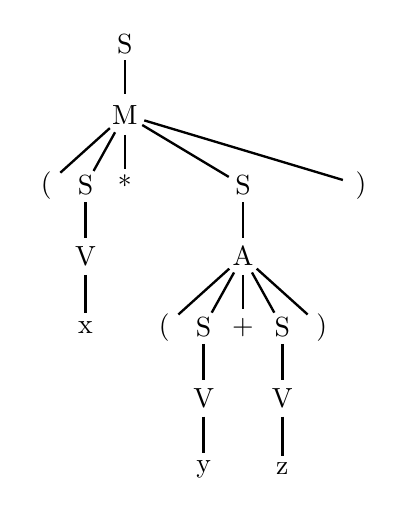
\begin{tikzpicture}[xscale=0.5,yscale=0.9,baseline={(current bounding box.center)}]
% \draw[help lines] (0,0) grid (7,2);
\node (s1) [circle,draw=none,inner sep=1pt] at (0,0) {\Snterm{S}};
{\node (s2) [circle,draw=none,inner sep=1pt] at (0,-1) {\Snterm{M}};}
{\node (s3) [circle,draw=none,inner sep=1pt] at (0,-2) {\Sterm{*}};
\node (s3a) [circle,draw=none,inner sep=1pt] at (3,-2) {\Snterm{S}};
\node (s3b) [circle,draw=none,inner sep=1pt] at (6,-2) {\Sterm{)}};
\node (s3x) [circle,draw=none,inner sep=1pt] at (-1,-2) {\Snterm{S}};
\node (s3y) [circle,draw=none,inner sep=1pt] at (-2,-2) {\Sterm{(}};}
{\node (s4) [circle,draw=none,inner sep=1pt] at (3,-3) {\Snterm{A}};}
{\node (s4z) [circle,draw=none,inner sep=1pt] at (-1,-3) {\Snterm{V}};}
{\node (s5) [circle,draw=none,inner sep=1pt] at (3,-4) {\Sterm{+}};
\node (s5a) [circle,draw=none,inner sep=1pt] at (4,-4) {\Snterm{S}};
\node (s5b) [circle,draw=none,inner sep=1pt] at (5,-4) {\Sterm{)}};
\node (s5x) [circle,draw=none,inner sep=1pt] at (2,-4) {\Snterm{S}};
\node (s5y) [circle,draw=none,inner sep=1pt] at (1,-4) {\Sterm{(}};}
{\node (s5z) [circle,draw=none,inner sep=1pt] at (-1,-4) {\Sterm{x}};}
{\node (s6a) [circle,draw=none,inner sep=1pt] at (4,-5) {\Snterm{V}};}
{\node (s6x) [circle,draw=none,inner sep=1pt] at (2,-5) {\Snterm{V}};}
{\node (s7a) [circle,draw=none,inner sep=1pt] at (4,-6) {\Sterm{z}};}
{\node (s7x) [circle,draw=none,inner sep=1pt] at (2,-6) {\Sterm{y}};}
% \node (s2) [circle,draw=none] at (0,3) {\Sterm{*}};
%
{\path[-,line width=0.3mm](s1) edge (s2);}
{\path[-,line width=0.3mm](s2) edge (s3);
\path[-,line width=0.3mm](s2) edge (s3a);
\path[-,line width=0.3mm](s2) edge (s3b);
\path[-,line width=0.3mm](s2) edge (s3x);
\path[-,line width=0.3mm](s2) edge (s3y);}
{\path[-,line width=0.3mm](s3x) edge (s4z);}
{\path[-,line width=0.3mm](s4z) edge (s5z);}
{\path[-,line width=0.3mm](s3a) edge (s4);}
{\path[-,line width=0.3mm](s4) edge (s5);
\path[-,line width=0.3mm](s4) edge (s5a);
\path[-,line width=0.3mm](s4) edge (s5b);
\path[-,line width=0.3mm](s4) edge (s5x);
\path[-,line width=0.3mm](s4) edge (s5y);}
{\path[-,line width=0.3mm](s5a) edge (s6a);}
{\path[-,line width=0.3mm](s5x) edge (s6x);}
{\path[-,line width=0.3mm](s6a) edge (s7a);}
{\path[-,line width=0.3mm](s6x) edge (s7x);}
% \path[->,line width=0.5mm](s1) edge node[below] {\Sterm{0}} (s2);
% \path[->,line width=0.5mm](s1) edge node[left] {\Sterm{1}} (s3);
% \path[->,line width=0.5mm](s3) edge node[right] {\Sterm{0}} (s2);
% \path[->,line width=0.5mm](s3) edge [loop above] node[above] {\Sterm{1}} (s3);
\end{tikzpicture}
\end{minipage}

\end{frame}

\begin{frame}\frametitle{Vom Ableitungsbaum zur Ableitung}

Beobachtung:
\begin{itemize}
\item Für jeden inneren Knoten im Ableitungsbaum gibt es genau einen Ableitungsschritt
\item Die Reihenfolge der Schritte ist egal, sofern Elternknoten vor ihren Kindern ersetzt werden
\end{itemize}\pause

\defbox{Eine totale Ordnung der Knoten eines Baums, bei der Eltern vor ihren Kindern betrachtet werden, heißt
\redalert{topologische Sortierung}.}

\begin{enumerate}[$\leadsto$]
\item Jede topologische Sortierung der Knoten eines Ableitungsbaumes führt zu einer erlaubten Ableitung
\end{enumerate}

\doodlebox{darkgreen}{\emph{Beispiel:}
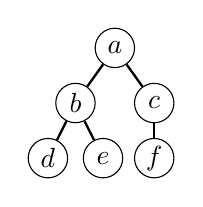
\begin{tikzpicture}[xscale=0.5,yscale=0.7,baseline=(s1.base)]
% \draw[help lines] (0,0) grid (7,2);
\node (s1) [circle,draw=black,inner sep=1pt,minimum height=5mm] at (0,0) {$a$};
\node (s2) [circle,draw=black,inner sep=1pt,minimum height=5mm] at (-1,-1) {$b$};
\node (s3) [circle,draw=black,inner sep=1pt,minimum height=5mm] at (1,-1) {$c$};
\node (s21) [circle,draw=black,inner sep=1pt,minimum height=5mm] at (-1.7,-2) {$d$};
\node (s22) [circle,draw=black,inner sep=1pt,minimum height=5mm] at (-0.3,-2) {$e$};
\node (s31) [circle,draw=black,inner sep=1pt,minimum height=5mm] at (1,-2) {$f$};
%
\path[-,line width=0.3mm](s1) edge (s2);
\path[-,line width=0.3mm](s2) edge (s21);
\path[-,line width=0.3mm](s2) edge (s22);
\path[-,line width=0.3mm](s1) edge (s3);
\path[-,line width=0.3mm](s3) edge (s31);
\end{tikzpicture}~~~
\begin{minipage}[t]{6.5cm}
Topologische Sortierungen:\\
$abcdef$ (Breitensuche von links), $acbfed$ (Breitensuche von rechts), $abdecf$ (Tiefensuche von links), $acfbed$ (Tiefensuche von rechts), \ldots
\end{minipage}
}

\end{frame}

\begin{frame}\frametitle{Vom Ableitungsbaum zur Ableitung: Beispiel}

Wir markieren die Variablen zur Veranschaulichung mit Indizes:\bigskip

\begin{minipage}{4.0cm}
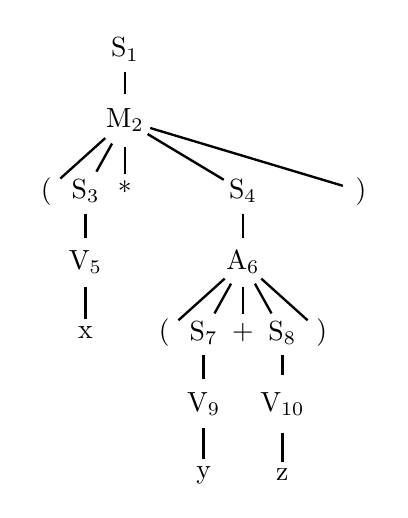
\begin{tikzpicture}[xscale=0.5,yscale=0.9,baseline={(current bounding box.center)}]
% \draw[help lines] (0,0) grid (7,2);
\node (s1) [circle,draw=none,inner sep=1pt] at (0,0) {\Snterm{S}${}_1$};
{\node (s2) [circle,draw=none,inner sep=1pt] at (0,-1) {\Snterm{M}${}_2$};}
{\node (s3) [circle,draw=none,inner sep=1pt] at (0,-2) {\Sterm{*}};
\node (s3a) [circle,draw=none,inner sep=1pt] at (3,-2) {\Snterm{S}${}_4$};
\node (s3b) [circle,draw=none,inner sep=1pt] at (6,-2) {\Sterm{)}};
\node (s3x) [circle,draw=none,inner sep=1pt] at (-1,-2) {\Snterm{S}${}_3$};
\node (s3y) [circle,draw=none,inner sep=1pt] at (-2,-2) {\Sterm{(}};}
{\node (s4) [circle,draw=none,inner sep=1pt] at (3,-3) {\Snterm{A}${}_6$};}
{\node (s4z) [circle,draw=none,inner sep=1pt] at (-1,-3) {\Snterm{V}${}_5$};}
{\node (s5) [circle,draw=none,inner sep=1pt] at (3,-4) {\Sterm{+}};
\node (s5a) [circle,draw=none,inner sep=1pt] at (4,-4) {\Snterm{S}${}_8$};
\node (s5b) [circle,draw=none,inner sep=1pt] at (5,-4) {\Sterm{)}};
\node (s5x) [circle,draw=none,inner sep=1pt] at (2,-4) {\Snterm{S}${}_7$};
\node (s5y) [circle,draw=none,inner sep=1pt] at (1,-4) {\Sterm{(}};}
{\node (s5z) [circle,draw=none,inner sep=1pt] at (-1,-4) {\Sterm{x}};}
{\node (s6a) [circle,draw=none,inner sep=1pt] at (4,-5) {\Snterm{V}${}_{10}$};}
{\node (s6x) [circle,draw=none,inner sep=1pt] at (2,-5) {\Snterm{V}${}_9$};}
{\node (s7a) [circle,draw=none,inner sep=1pt] at (4,-6) {\Sterm{z}};}
{\node (s7x) [circle,draw=none,inner sep=1pt] at (2,-6) {\Sterm{y}};}
% \node (s2) [circle,draw=none] at (0,3) {\Sterm{*}};
%
{\path[-,line width=0.3mm](s1) edge (s2);}
{\path[-,line width=0.3mm](s2) edge (s3);
\path[-,line width=0.3mm](s2) edge (s3a);
\path[-,line width=0.3mm](s2) edge (s3b);
\path[-,line width=0.3mm](s2) edge (s3x);
\path[-,line width=0.3mm](s2) edge (s3y);}
{\path[-,line width=0.3mm](s3x) edge (s4z);}
{\path[-,line width=0.3mm](s4z) edge (s5z);}
{\path[-,line width=0.3mm](s3a) edge (s4);}
{\path[-,line width=0.3mm](s4) edge (s5);
\path[-,line width=0.3mm](s4) edge (s5a);
\path[-,line width=0.3mm](s4) edge (s5b);
\path[-,line width=0.3mm](s4) edge (s5x);
\path[-,line width=0.3mm](s4) edge (s5y);}
{\path[-,line width=0.3mm](s5a) edge (s6a);}
{\path[-,line width=0.3mm](s5x) edge (s6x);}
{\path[-,line width=0.3mm](s6a) edge (s7a);}
{\path[-,line width=0.3mm](s6x) edge (s7x);}
% \path[->,line width=0.5mm](s1) edge node[below] {\Sterm{0}} (s2);
% \path[->,line width=0.5mm](s1) edge node[left] {\Sterm{1}} (s3);
% \path[->,line width=0.5mm](s3) edge node[right] {\Sterm{0}} (s2);
% \path[->,line width=0.5mm](s3) edge [loop above] node[above] {\Sterm{1}} (s3);
\end{tikzpicture}
\end{minipage}\hfill
\begin{minipage}{5.7cm}
% Grammatik:
% \begin{align*}
% \Snterm{S} &\to \Snterm{A}\mid \Snterm{M}\mid \Snterm{V} &
% \Snterm{A} &\to \Sterm{(}\Snterm{S}\Sterm{+}\Snterm{S}\Sterm{)} \\
% \Snterm{M} &\to \Sterm{(}\Snterm{S}\Sterm{*}\Snterm{S}\Sterm{)} &
% \Snterm{V} &\to \Sterm{x}\mid\Sterm{y}\mid\Sterm{z}
% \end{align*}
% 
\pause
Sortierung $\Snterm{S}_1\Snterm{M}_2\Snterm{S}_3\Snterm{V}_5\Snterm{S}_4\Snterm{A}_6\Snterm{S}_7\Snterm{V}_9\Snterm{S}_8\Snterm{V}_{10}$:\vspace{-1ex}
\begin{align*}
\Snterm{S}_1 & \Rightarrow \Snterm{M}_2
	\Rightarrow \Sterm{(}\Snterm{S}_3\Sterm{*}\Snterm{S}_4\Sterm{)}
	\Rightarrow \Sterm{(}\Snterm{V}_5\Sterm{*}\Snterm{S}_4\Sterm{)}\\
	&\Rightarrow \Sterm{(}\Sterm{x}\Sterm{*}\Snterm{S}_4\Sterm{)}
	\Rightarrow \Sterm{(}\Sterm{x}\Sterm{*}\Snterm{A}_6\Sterm{)}\\
	&\Rightarrow \Sterm{(}\Sterm{x}\Sterm{*}\Sterm{(}\Snterm{S}_7\Sterm{+}\Snterm{S}_8\Sterm{)}\Sterm{)}
	\Rightarrow \Sterm{(}\Sterm{x}\Sterm{*}\Sterm{(}\Snterm{V}_9\Sterm{+}\Snterm{S}_8\Sterm{)}\Sterm{)}\\
	&\Rightarrow \Sterm{(}\Sterm{x}\Sterm{*}\Sterm{(}\Sterm{y}\Sterm{+}\Snterm{S}_8\Sterm{)}\Sterm{)}
	\Rightarrow \Sterm{(}\Sterm{x}\Sterm{*}\Sterm{(}\Sterm{y}\Sterm{+}\Snterm{V}_{10}\Sterm{)}\Sterm{)}\\
	&\Rightarrow \Sterm{(}\Sterm{x}\Sterm{*}\Sterm{(}\Sterm{y}\Sterm{+}\Sterm{z}\Sterm{)}\Sterm{)}
\end{align*}\vspace{-4ex}\pause

Entspricht Tiefensuche von links\\
$\leadsto$ \redalert{Linksableitung}
\bigskip

\pause
Alternative Reihenfolge bei Tiefensuche von rechts:

$\Snterm{S}_1\Snterm{M}_2\Snterm{S}_4\Snterm{A}_6\Snterm{S}_8\Snterm{V}_{10}\Snterm{S}_7\Snterm{V}_9\Snterm{S}_3\Snterm{V}_5$\\
$\leadsto$ \redalert{Rechtsableitung}

% Alternative Ableitung:\vspace{-2ex}
% \begin{align*}
% \Snterm{S} & \Rightarrow \Snterm{M}
% 	\Rightarrow \Sterm{(}\Snterm{S}\Sterm{*}\Snterm{S}\Sterm{)}
% 	\Rightarrow \Sterm{(}\Snterm{S}\Sterm{*}\Snterm{A}\Sterm{)} \\
% 	& \Rightarrow \Sterm{(}\Snterm{S}\Sterm{*}\Sterm{(}\Snterm{S}\Sterm{+}\Snterm{S}\Sterm{)}\Sterm{)}
% 	\Rightarrow \Sterm{(}\Snterm{S}\Sterm{*}\Sterm{(}\Snterm{S}\Sterm{+}\Snterm{V}\Sterm{)}\Sterm{)} \\
% 	& \Rightarrow \Sterm{(}\Snterm{S}\Sterm{*}\Sterm{(}\Snterm{V}\Sterm{+}\Snterm{V}\Sterm{)}\Sterm{)} 
% 	\Rightarrow \Sterm{(}\Snterm{V}\Sterm{*}\Sterm{(}\Snterm{V}\Sterm{+}\Snterm{V}\Sterm{)}\Sterm{)} \\
% 	& \Rightarrow \Sterm{(}\Snterm{V}\Sterm{*}\Sterm{(}\Snterm{V}\Sterm{+}\Sterm{z}\Sterm{)}\Sterm{)} 
% 	 \Rightarrow \Sterm{(}\Snterm{V}\Sterm{*}\Sterm{(}\Sterm{y}\Sterm{+}\Sterm{z}\Sterm{)}\Sterm{)} \\
% 	& \Rightarrow \Sterm{(}\Sterm{x}\Sterm{*}\Sterm{(}\Sterm{y}\Sterm{+}\Sterm{z}\Sterm{)}\Sterm{)}
% \end{align*}\vspace{-1ex}
\end{minipage}

\end{frame}

\begin{frame}\frametitle{Rechtsableitungen und Linksableitungen}

Man kann diese speziellen Ableitungen auch ohne den Ableitungsbaum direkt erzeugen:
\begin{itemize}
\item \redalert{Linksableitung:} In jedem Ableitungsschritt wird die am weitesten links stehende Variable ersetzt
\item \redalert{Rechtsableitung:} In jedem Ableitungsschritt wird die am weitesten rechts stehende Variable ersetzt
\end{itemize}
\bigskip

Bei CFGs kann jede dieser Strategien jedes erzeugbare Wort generieren\\[1ex]
(bei Typ-1-Grammatiken im Allgemeinen nicht -- Übung: warum?)

\end{frame}



\begin{frame}\frametitle{Anwendung Ableitungsbaum}

Der Ableitungsbaum ist von großer praktischer Bedeutung, 
da er die \alert{"`innere Struktur"'} eines Wortes einer kontextfreien Sprache
repräsentiert
\bigskip

% \begin{enumerate}[$\leadsto$]
% \item
\anybox{purple}{%
In der Praxis geht es meist nicht darum, zu prüfen, ob ein Wort in einer Sprache liegt, sondern darum, seine
syntaktische Struktur zu ermitteln}%
% \end{enumerate}
\bigskip

\emph{Beispiele:}
\begin{itemize}
\item Parsebäume in der \alert{Verarbeitung natürlicher Sprache} können Aufschluss über die Bedeutung eines Satzes geben
\item Syntaxbäume in \alert{Programmiersprachen} sind die Grundlage für die inhaltliche Interpretation des Codes
\item Ableitungsbäume in \alert{Mark-Up-Sprachen} wie HTML oder XML sind entscheidend für die Adressierung von Elementen ("`DOM-Tree"')
\end{itemize}

\end{frame}

\begin{frame}\frametitle{Zusammenfassung und Ausblick}

Wir kennen \redalert{viele Charakterisierungen für reguläre Sprachen}, die man mit zahlreichen Umformungen in Beziehung setzen kann\bigskip

% Die wichtigsten Ideen und Methoden der Vorlesungen zu regulären Sprachen lassen sich auf wenigen Folien zusammenfassen, aber
% \bigskip

Wörter in \redalert{kontextfreien Sprachen} haben eine interessante innere Struktur, die wir durch \redalert{Ableitungsbäume} darstellen können\bigskip

Bei Typ-2-Grammatiken repräsentieren Ableitungsbäume mehrere mögliche Ableitungen.\bigskip

\anybox{yellow}{
Offene Fragen:
\begin{itemize}
\item Wie kann das Wortproblem bei kontextfreien Grammatiken gelöst werden?
\item Haben kontextfreie Sprachen ein Berechnungsmodell?
\item Wie sehen nichtkontextfreie Sprachen aus und wie erkennt man sie?
\end{itemize}
}

\end{frame}


\end{document}
